
\documentclass[UTF8,a4paper]{ctexart}
\usepackage[margin=20mm,top=21mm,bottom=20mm]{geometry}
\usepackage{amsmath,amssymb,booktabs,tabularx,graphicx,xcolor,fancyhdr,enumitem,tikz}
\usetikzlibrary{arrows.meta,positioning}
\usepackage[colorlinks=true,linkcolor=teal,urlcolor=teal]{hyperref}
\definecolor{ink}{HTML}{142B43}\definecolor{accent}{HTML}{168579}
\pagestyle{fancy}\fancyhf{}\fancyhead[L]{\small\color{ink}CF2026 · Project 1}\fancyhead[R]{\small 青序量化研究平台}
\fancyfoot[L]{\scriptsize 真实数据快照 · 描述性研究 · 源码版本 9dd8c3f}\fancyfoot[R]{\thepage/8}
\setlength{\headheight}{14pt}\setlength{\parindent}{2em}\setlength{\parskip}{4pt}
\setlist{nosep,leftmargin=1.8em}
\ctexset{section={format=\Large\bfseries\color{ink}},subsection={format=\normalsize\bfseries\color{accent}}}
\newcommand{\pct}[1]{#1\%}
\newcommand{\lead}[1]{\noindent{\color{accent}\bfseries #1}\par}
\begin{document}
\begin{center}
{\small\color{accent}COMPUTATIONAL FINANCE / RESEARCH INFRASTRUCTURE}\\[8pt]
{\Huge\bfseries\color{ink}青序量化研究平台}\\[7pt]
{\large 从真实行情到可核验的研究结论}\\[8pt]
2026年9月21日\quad 研究区间：2023--2025\\
{\small 小组成员：待填写}
\end{center}
\section*{1\quad 目标与设计选择}
\lead{先完成正确的研究闭环，再接入更复杂的预测模型。}
本项目建立可维护、可扩展的日频量化研究平台，覆盖数据快照、质量检查、三个因子、目标组合、含成本成交、净值与风险分析。对齐课件的完整性、正确性、可复现性及可扩展性要求；不以收益、Sharpe或IC达到某个阈值作为成功条件。

选择Python，复用pandas/NumPy/SciPy处理面板与统计，Plotly和Streamlit提供交互。计算包与界面分离，命令行和界面调用同一核心。检查了Backtrader、Alphalens和Qlib：本项目复用Backtrader作独立参考测试；为保持课程的缺失、并列、成交和会计口径显式可查，主账本采用小型透明实现。

\begin{center}
\begin{tikzpicture}[node distance=5mm and 5mm,box/.style={draw=accent!50,fill=accent!5,rounded corners,minimum width=42mm,minimum height=11mm,font=\small},>=Stealth]
\node[box](a){数据与快照};
\node[box,right=of a](b){因子与目标组合};
\node[box,right=of b](c){成交与现金账本};
\node[box,below=of c](d){净值与绩效};
\node[box,left=of d](e){诊断与对照实验};
\node[box,left=of e](f){复现包与交互界面};
\draw[->](a)--(b);\draw[->](b)--(c);\draw[->](c)--(d);\draw[->](d)--(e);\draw[->](e)--(f);
\end{tikzpicture}
\end{center}

\subsection*{论文参考如何进入本次工程}
CogAlpha研究LLM驱动的因子代码生成、质量检查及进化搜索。本项目借鉴因子卡、可注册代码与时间泄漏检查，未实现其多智能体生成流程，也不声称复现论文收益。神经网络留作后续可替换的信号模块；它不能替代数据、现金和成本核算。

\subsection*{本次成果与验收入口}
\noindent\begin{tabularx}{\linewidth}{lX}
\toprule
层次 & 可检查证据\\\midrule
数据 & 原始请求缓存、标准行情、日历、质量报告、校验清单\\
算法 & 三因子公式与长表、下一开盘执行、成本及逐日账本\\
研究 & 三因子诊断、5日/20日调仓对照、真实亏损结果\\
工程 & 独立模块、测试、中文界面、命令行、Git分阶段提交\\
\bottomrule
\end{tabularx}

\newpage
\section*{2\quad 研究样本与数据质量}
\lead{股票池由研究开始前的数据确定，之后不按表现删除资产。}
以2022年12月30日为选池日：主板代码前缀000/001/002/003/600/601/603/605，收盘价至少3元、成交量大于零，按当日成交额选前60只，并列按代码。未以当前仍上市为条件，也未按未来收益筛选。该规则偏向当时交易活跃的股票，不代表全市场或历史沪深300。

通过用户已有Tushare权限获取daily、adj\_factor、stk\_limit、trade\_cal。下载2022年10月至2025年末，首段用于因子预热。研究区间含727个交易日。原始请求记录参数与UTC时间，成功缓存可复用，凭据不保存到项目或Git中。

\begin{center}
\begin{tabular}{lr}\toprule
检查项 & 本次快照结果\\\midrule
资产数 & 60\\
日历交易日（含预热） & 787\\
原始记录 / 标准记录 & 46,759 / 46,759\\
重复日期--资产键 & 0\\
不合法价格、成交量排除行 & 0\\
相对于全日历网格的缺失记录 & 461\\
已有行情行中缺失涨跌停价格 & 0\\\bottomrule
\end{tabular}
\end{center}
461个缺口包含上市前、停牌或其他缺失，不能全部解释为数据错误。保留缺口，不统一填零，不用未来价格反填。缺失行情的持仓单独记录，长期缺失使用第4页的保守估值规则。

\subsection*{字段与复权口径}
\noindent\begin{tabularx}{\linewidth}{lX}\toprule
字段 & 定义\\\midrule
date / asset & 交易日与证券代码，联合唯一键\\
raw\_open / raw\_close & 原始开收盘价，元/股；原始高低价也保留\\
adj\_factor & 厂商累计乘法复权因子\\
open / high / low / close & 固定参考尺度的复权OHLC\\
volume & 股；Tushare原始vol以手计，导入乘100\\
up\_limit / down\_limit & 原始价格尺度的当日上下限\\\bottomrule
\end{tabularx}
\[
P^{\mathrm{adj}}_{i,t}=P^{\mathrm{raw}}_{i,t}\frac{a_{i,t}}{a_{i,\tau_i}},
\]
其中$\tau_i$是本快照该资产的首个有效日期，整个样本保持固定。OHLC使用同一调整比例。复权总收益单位近似分红再投资，不等同于真实股东分红现金账。

\subsection*{数据局限}
没有完整历史ST过滤、行业中性化或逐时点厂商版本；后来下载的快照可能含历史修订。固定资产池可能集中于选池日热点。数据与许可范围保留在本地，Git只包含合成演示与汇总证据。

\newpage
\section*{3\quad 三个因子与统一接口}
设$C_{i,t}$为复权收盘价，$r_{i,t}=C_{i,t}/C_{i,t-1}-1$。统一规定分数越高，预期收益越高；这一方向事先固定，即使结果不支持也不翻转。

\subsection*{20日动量}
\[
f^{\mathrm{mom}}_{i,t}=C_{i,t}/C_{i,t-20}-1.
\]
假设近期相对强势可能延续。输入为收盘价，要求窗口内21个价格完整。震荡反转、拥挤交易及趋势突变可能使其失效。

\subsection*{5日反转}
\[
f^{\mathrm{rev}}_{i,t}=-\left(C_{i,t}/C_{i,t-5}-1\right).
\]
假设短期下跌后可能反弹。要求窗口内6个价格完整。若下跌来自持续基本面恶化，或者趋势较强，则反转假设可能失败。

\subsection*{20日低波动}
\[
f^{\mathrm{lowvol}}_{i,t}
=-\operatorname{std}_{\mathrm{sample}}(r_{i,t-19},\ldots,r_{i,t}),
\quad \mathrm{ddof}=1.
\]
负号将低风险方向转换为高分。窗口20个收益均需有效；快涨阶段可能落后，行业或风格暴露可能混淆解释。本次不做去极值、中性化或全样本标准化。

\subsection*{窗口不能跨过缺口偷换含义}
先对齐完整交易日历，再滚动计算；缺失不前填，也不删除停牌日后把“20个观测”当作“20个交易日”。预热不足的因子为缺失。输出长表为date、asset、factor、value，因子公式不进入成交模块。

\subsection*{信号与未来标签的时间关系}
在$t$日收盘后形成分数，最早在$t+1$开盘成交。诊断标签采用：
\[
y^{(h)}_{i,t}=\frac{O^{\mathrm{adj}}_{i,t+1+h}}
                         {O^{\mathrm{adj}}_{i,t+1}}-1,\qquad h=5.
\]
标签只用于评价，绝不输入目标权重。研究结束之后的价格不参与诊断；最后6个形成日自然没有完整5日标签。标签端点有效不意味着它一定能在市场限制下成交。

\subsection*{插件扩展与泄漏检测}
注册表保存名称、公式、假设、默认窗口、失效条件与计算函数。新增因子保留日期/资产轴即可复用诊断和回测。测试同时使用截断重算与未来价格扰动，要求过去因子不变，并通过一个故意使用未来值的插件验证检测能失败。这是实用检查，不是任意模型的绝对安全证明。

\newpage
\section*{4\quad 组合、成交与会计核验}
\lead{可执行组合净值来自账本，不能用重叠标签直接连乘。}
基准策略每5个交易日调仓，选择上一交易日分数最高的10只等权，并列按代码。无分数时目标现金，不足10只时对现有分数等权。调仓从研究首日计数；“周度/月度”仅是5/20交易日的简称，不是自然周/月末。

在当前开盘报价下确定名义金额和研究单位，先卖后买。为避免满仓目标挤占费用，目标总名义预算为
\[
V_t^-/(1+c_b+c_s).
\]
卖单受阻使现金不足时，对当日可执行买单等比例缩减。未成交订单当日失效，下次调仓重新计算，不自动排队。实际持仓可能因旧仓无法卖出而超过目标数量。

\subsection*{市场限制与费用}
开盘价缺失不成交；原始开盘价达到涨停时不买入，达到跌停时不卖出；对应限制价缺失也不成交。该日频规则是保守近似，未描述订单队列。
\[
\mathrm{Cost}_t=c_bB_t+c_sS_t,\quad
c_b=0.001,\quad c_s=0.0015.
\]
买10bp、卖15bp为固定研究假设，不是对历史实际税费的声明。仅按真实模拟成交额$B_t,S_t$扣费，无成交不收费。未建模最低佣金、整手、冲击成本或容量。

\subsection*{缺失与长期估值风险}
缺失收盘时沿用最后有效收盘估值并记录陈旧持仓；连续超过20个交易日缺失后保守计零，单位仍保留，报价恢复再估值。该规则不是已确认退市或清偿价值，不生成假卖出与费用。总净值非正则停止报错。

\subsection*{净值与独立复核}
\[
V_t=\mathrm{Cash}_t+\sum_i q_{i,t}P^{\mathrm{mark}}_{i,t},\qquad
\mathrm{Turnover}_t=\frac{B_t+S_t}{V_t^-}.
\]
这是连续可分的复权总收益单位$q$，而非真实交易股数。独立复核从成交重新累积现金和单位，核对持仓、市值、净值、费用、信号先后与收益连乘；现金绝不透支，不能做空。

绩效以扣费后为主：累计收益$V_N/V_0-1$，年化收益$(V_N/V_0)^{252/N}-1$，年化波动$\sqrt{252}\operatorname{std}(R)$，Sharpe为日超额收益均值除样本标准差再乘$\sqrt{252}$。无风险年收益默认0，期初$V_0$进入首日收益与回撤高水位。

毛归因采用相同成交路径，向不计息现金退回累计费用，即$V_t^{\mathrm{gross}}=V_t+\sum_{s\le t}\mathrm{Cost}_s$；它不是重新投资的无成本策略。

\newpage
\section*{5\quad 因子诊断：信息不等于利润}
在每个形成日跨资产计算Pearson IC与Spearman Rank IC，再沿时间汇总。Spearman并列平均秩，至少10个有效配对；常数或不足样本记缺失，不写成零。有效诊断日均为721天。

\begin{center}\small
\begin{tabular}{lrrrrr}\toprule
因子 & IC均值 & IC标准差 & Rank IC均值 & Rank IC标准差 & 覆盖率\\\midrule
动量 & -0.0669 & 0.2608 & -0.0634 & 0.2275 & 98.24\% \\
反转 & 0.0471 & 0.2447 & 0.0371 & 0.2144 & 98.88\% \\
低波动 & 0.0404 & 0.2519 & 0.0777 & 0.2482 & 98.24\% \\
\bottomrule\end{tabular}
\end{center}

\noindent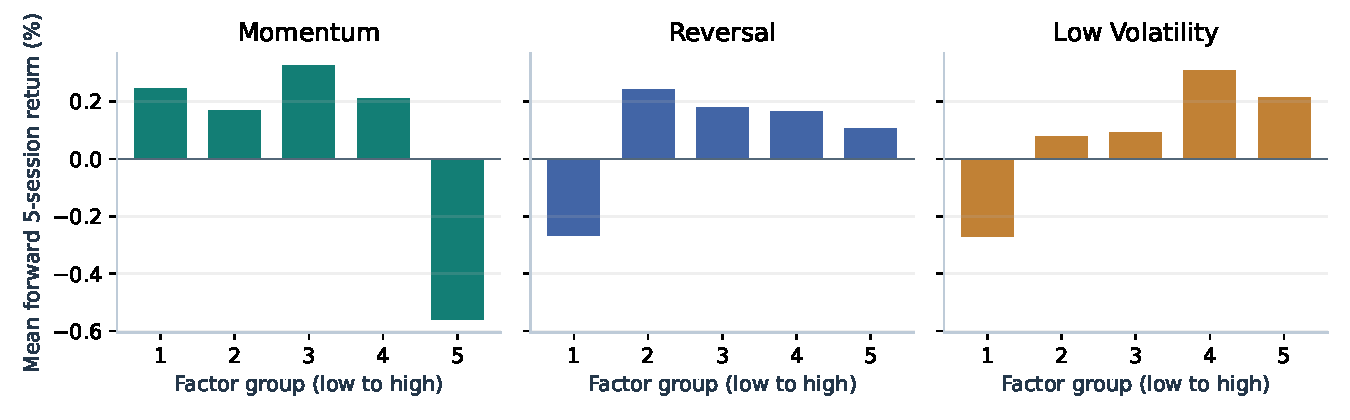
\includegraphics[width=\linewidth]{figures/groups.pdf}
\begin{center}\small 图1：按当日因子从低到高分为五组，比较未来5日平均收益。\end{center}

分组先由形成日的有效分数决定，并列按资产代码稳定排序；之后才匹配未来标签。标签缺失时报告原始组人数与有效人数，不重新分组。组间价差没有扣费，不代表可执行多空收益，更不能将重叠5日标签连乘成策略净值。

\subsection*{结果解释}
动量的平均IC和Rank IC均为负，最高组相对最低组的5日期望差约为$-0.8062$个百分点，本样本不支持预设动量方向。反转平均IC为正，组间差约为$0.3724$个百分点；低波动组间差约为$0.4827$个百分点。

这些结果回答的是横截面排序问题。真正策略还涉及只买最高组、调仓、市场限制与费用。反转即使有正IC，也可能因高换手及路径风险出现负的净收益。IC=0.05不等于5\%收益，也不等于55\%预测正确率。

\subsection*{统计解释的边界}
5日标签重叠，日序列存在相关性。本次不做未经适当修正的显著性声明，也不据此宣称新的alpha发现。固定样本与风格暴露可能解释部分现象；因子方向和窗口均未为改善这些结果而事后调整。

\newpage
\section*{6\quad 真实净值与风险}
\begin{center}\small
\begin{tabular}{lrrrrr}\toprule
策略 & 累计收益 & 年化收益 & Sharpe & 最大回撤 & 总费用/万元\\\midrule
动量/5日 & -64.60\% & -30.23\% & -1.092 & 72.88\% & 7.90 \\
反转/5日 & -49.71\% & -21.20\% & -0.675 & 62.12\% & 17.85 \\
低波动/5日 & 24.84\% & 7.99\% & 0.545 & 18.66\% & 8.90 \\
动量/20日 & -41.31\% & -16.87\% & -0.571 & 57.41\% & 4.52 \\
\bottomrule\end{tabular}
\end{center}
\noindent
\includegraphics[width=\linewidth]{figures/nav.pdf}
\begin{center}\small 图2：相同期初100万元，保留所有净值路径，包括明显亏损的基线。\end{center}
\noindent
\includegraphics[width=\linewidth]{figures/drawdown.pdf}
\begin{center}\small 图3：相对包括初始资金在内的历史高水位计算回撤。\end{center}
\subsection*{如何读取结果}
三种因子共享相同数据、费用和执行模块。低波动在本样本中的表现相对较好，不构成对未来最佳策略的选择结论。反转产生更高换手，累计费用显著高于动量；这里总费用以实际金额报告，不能单独用它排序成本效率，因为资金路径不同。

\newpage
\section*{7\quad 控制变量实验与软件证据}
\lead{事前问题：仅延长调仓间隔，能否降低换手与费用？}
动量因子、20日窗口、股票池、样本期、目标10只、初始资金和成本均保持不变；仅将调仓间隔由5改为20个交易日。预期交易频率与成本下降，对收益和风险方向不作预设。

\noindent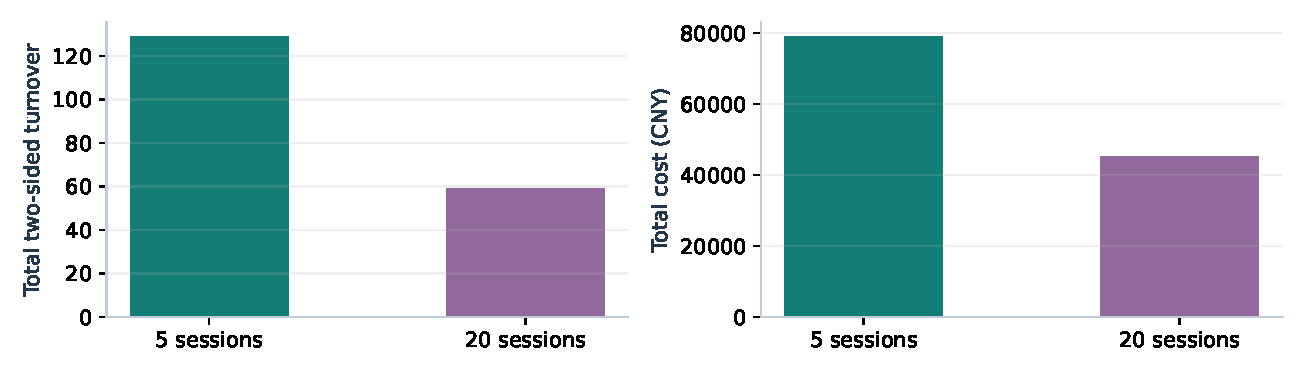
\includegraphics[width=\linewidth]{figures/comparison.pdf}
\begin{center}\small 图4：唯一主变量为调仓间隔；成本与换手使用相同定义。\end{center}

累计双边换手从128.88降到59.10；总费用从79,002.49元降到45,170.43元，下降42.82\%。净累计收益从-64.60\%变为-41.31\%，但两者均亏损。延长持有减少了交易成本，也改变了持仓暴露与路径，不能把收益差全部归因于费用。

该对照支持“低频调仓减少本样本交易负担”，不证明低频一般更好。毛归因口径只是同路径费用归还，可以辅助解释，却不是严格固定暴露下的因果分解。

\subsection*{验收不只看图}
\noindent\begin{tabularx}{\linewidth}{lX}\toprule
检查 & 证据\\\midrule
公式手算 & 三因子、下一开盘标签、费用与换手、初始高水位回撤\\
成交限制 & 缺失开盘、涨跌停单边阻止、现金约束和陈旧估值\\
公司行动 & 二拆一时复权单位净值保持连续\\
防泄漏 & 三因子前缀/未来扰动；故意泄漏插件被检测\\
独立参考 & Backtrader单资产固定交易/持有结果与本账本一致\\
复现 & 同快照配置两次主基准净值与成交完全一致\\
扩展 & 注册区间振幅因子，无需修改成交核心\\\bottomrule
\end{tabularx}

数值账本容差：现金绝对$10^{-6}$元、相对$10^{-10}$。自动测试与GitHub Actions日志随代码可查，交互页面另经参数提交检查。任何新增模型需增加适合其风险的测试，不能把当前测试结果当作未来代码的保证。

\newpage
\section*{8\quad 复现、拓展与局限}
\subsection*{复现最短路径}
\begin{enumerate}
\item 安装Python3.12/3.13，用requirements-lock.txt安装固定直接依赖，执行pip install -e .。
\item 通过本地凭据运行下载入口，或恢复获准使用的本地行情快照。核对manifest.json。
\item 运行python -m cfquant.cli study，生成三因子、主对照和复核结果。
\item 运行python -m pytest -q；启动launch.cmd检查交互界面。
\end{enumerate}
无凭据时可运行configs/demo.yaml中的合成样本，但它仅验证软件可用，不是本报告真实实证的替代。

\noindent 本次行情SHA-256：\\
{\ttfamily\scriptsize 1490ae85e156920d930c81e482f2a8a2ba8353e150d58fc224d92d49d35b6ddc}

每次实验记录Git版本、源文件哈希、数据与日历哈希、完整配置、UTC时间、耗时和检查输出。原始行情与Token不进入Git，仓库保留可分享合成样本与汇总证据。本地完整快照和报告源码随交付包保存。

\subsection*{可维护性与后续项目}
数据提供者、因子注册、组合权重、成交账本、诊断和UI分别承担单一职责。后续新增因子只修改插件；预测模型在独立训练模块完成，将样本外分数送入现有接口。需要按时间划分数据、清除跨边界标签，避免全样本标准化。神经网络是否有益，应与简单模型在同一未触碰测试期比较。

\subsection*{尚未覆盖的内容}
本平台是研究级模拟。未完整建模整手、股东现金分红、税费历史变化、最低佣金、盘口、订单排队和容量冲击。开盘按目标名义金额再平衡较理想化；长期缺失计零具有主观性。固定热点股票池、厂商历史修订和未中性化风格暴露限制外推。没有宣称显著alpha、投资建议或实盘可直接部署。

\subsection*{主要来源}
\begin{enumerate}\small
\item 课程文件：CF2026\_Project1.pdf，19页，评分、公式与交付要求。
\item Liu et al. \textit{Cognitive Alpha Mining via LLM-Driven Code-Based Evolution}, arXiv:2511.18850v4。参考其因子表示与质量检查。
\item Tushare官方接口：\url{https://tushare.pro/document/2?doc_id=27}（日线），doc\_id=28（复权），183（涨跌停），26（日历）。
\item Backtrader：\url{https://github.com/mementum/backtrader}；Alphalens：\url{https://github.com/quantopian/alphalens}；Qlib：\url{https://github.com/microsoft/qlib}。
\item CogAlpha作者提示词仓库：\url{https://github.com/uwFengyuan/CogAlpha_Prompt}。
\end{enumerate}
\end{document}
